%%%%
% Consiglio la visione dei seguenti tutorial:
% - https://www.youtube.com/watch?v=ihxSUsJB_14
% - https://www.youtube.com/watch?v=XTFWaV55uDo
%%%%
\documentclass[12pt,a4paper,openright,twoside]{book}
\usepackage[utf8]{inputenc}

%\newcommand{\thesislang}{italian} % decommentare in caso di tesi in italiano
\newcommand{\thesislang}{english} % commentare in caso di tesi in italiano
\usepackage{thesis-style}
% version
\newcommand{\versionmajor}{0}
\newcommand{\versionminor}{1}
\newcommand{\versionpatch}{2}
\newcommand{\version}{\versionmajor.\versionminor.\versionpatch}
\typeout{Document version: \version}

\begin{document}
	
\frontmatter

% ! TeX root = thesis-main.tex
\title{Title}
\author{Candidate Name Here}
\date{\today}

\newgeometry{margin=0.8in}
\begin{titlepage}
	\begin{center}
		% \vspace*{0.2cm}
		
		\large
		\textbf{ALMA MATER STUDIORUM -- UNIVERSITÀ DI BOLOGNA \\ CAMPUS DI CESENA}
		\\
		\noindent\hrulefill
		\vspace{0.4cm}
		
		\Large
		Scuola di Ingegneria e Architettura \\
		Corso di Laurea Magistrale in Ingegneria e Scienze Informatiche
		
		\Huge
		\vspace{4cm}
		\textbf{
			Aggregate Computing and Many-Agent Reinforcement Learning: 
			Towards a Hybrid Approach
		}
		
		\large
		\vspace{1cm}
		Tesi di laurea in 
		\\ 
		\textsc{Pervasive Computing}
		
		\vspace{5.5cm}
		\begin{minipage}[t]{0.64\textwidth}
			\begin{flushleft}
				\textit{Relatore} 
				\\ 
				\textbf{Prof.} \textbf{Mirko Viroli}
				\\
				\vspace{0.4cm}
				\textit{Correlatore} 
				\\
				\textbf{Dott.} \textbf{Gianluca Aguzzi}
			\end{flushleft}
		\end{minipage}
		\begin{minipage}[t]{0.34\textwidth}
			\begin{flushright}
				\textit{Candidato} 
				\\ 
				\textbf{Davide Domini}
			\end{flushright}
		\end{minipage}\\
		
		\vfill
		\noindent\hrulefill
		\vspace{0.3cm}
		\Large
		
		Seconda Sessione di Laurea
		\\
		Anno Accademico 2022-2023
	\end{center}
\end{titlepage}
\restoregeometry


\begin{abstract}	
Max 2000 characters, strict.
\end{abstract}

\begin{dedication} 
Optional. Max a few lines.
\end{dedication}

\begin{acknowledgements}
Optional. Max 1 page.
\end{acknowledgements}

%----------------------------------------------------------------------------------------
\tableofcontents   
\listoffigures     
\lstlistoflistings 
%----------------------------------------------------------------------------------------

\mainmatter

%----------------------------------------------------------------------------------------
\chapter{\introductionname}
\label{chap:introduction}
%----------------------------------------------------------------------------------------


\paragraph{Thesis motivation} % TODO --- Riformulare e approfondire meglio

Significant technological advancements have paved the way for the emergence of a field known as \emph{Collective Computing} 
    \cite{abowd2016beyond}, with \emph{Cyber-Physical Swarms (CPSW)} \cite{schranz2021swarm} as a noteworthy branch within it.
    The latter consist of myriad devices that interact with the environment and exchange information among themselves. 
    A crucial aspect of these systems is that a more complex collective behavior emerges from the interaction between 
    individual agents that leads to the resolution of various tasks.
    Among all aspects related to CPSW, our focus lies on properties like \emph{collective intelligence} \cite{tumer2004survey} 
    and \emph{self-organization} \cite{schmeck2011organic}. This stems from the applications of these systems, leading us to 
    concentrate on their collective behavior to express autonomy, adaptability, and coordination of the devices 
    that are part of them.

This progress has been driven by research in various related fields such as: multi-agent systems \cite{dorri2018multi},
     coordination \cite{yang2022overview}, distributed artificial intelligence \cite{bond2014readings}, and many others. 
     Additionally, it has a profound impact on a wide range of applied domains, including: smart cities \cite{zedadra2019swarm}, 
     swarm robotics \cite{brambilla2013swarm}, large-scale IoT systems \cite{uslu2023role}, and more.

A crucial aspect to consider in CPSW is how individual devices are programmed and achieve coordination to perform assigned tasks. 
Novel approaches -- like \emph{aggregate computing} \cite{viroli2018field} -- have focused on manually developing
controllers from a global perspective. However, this approach has some drawbacks: it is highly challenging to write satisfactory 
and efficient programs for complex tasks, they may be error-prone and lack of generality.

On the other hand, there exists approaches that leverage various artificial intelligence (AI) techniques, 
such as \emph{Multi-Agent Reinforcement Learning} (MARL) \cite{busoniu2008comprehensive},
to enable devices to learn directly from experience and/or data. These approaches also present several challenges, including: non-stationarity 
\cite{hernandez2017survey}, communication and scalability.

%
\paragraph{Thesis objectives}

Starting from what was seen in the previous paragraph, the goal of this thesis is to lay the foundation for a hybrid approach 
    that can succeed in exploiting the potential of both macro-programming, in particular \emph{aggregate computing} is taken as a 
    reference, and AI approach.
    In order to achieve this goal, it is necessary to develop a toolchain that allows these systems to be developed in an agile,
    fast and reusable way. 
    Scarlib, whose development has already started in \cite{scarlib}, is the tool that for us forms the basis of this toolchain.
    Its main purpose is to integrate the \emph{ScaFi} \cite{casadei2022scafi} (an implementation of aggregate computing) 
    and \emph{Alchemist} \cite{pianini2013chemical} (a bio-chemical based simulator) tools with \emph{Reinforcement Learning} 
    to help develop experiments in \emph{simulated} environments with \emph{offline learning}.

%
\paragraph{Thesis Structure} 


%----------------------------------------------------------------------------------------
\chapter{Background}
\label{chap:background}
%----------------------------------------------------------------------------------------

\section{Cyber-Physical Swarms}
%
\section{Aggregate Computing}

The advent of \emph{Collective Computing} and the proliferation of interconnected devices have given rise to novel 
    paradigms that aim to address the challenges posed by the distributed nature of computing
    systems. One such paradigm that has gained significant attention in recent years is 
    \emph{aggregate computing (AC)} [8].

AC is well grounded on \emph{field calculus}, and therefore adopts a model where the perspective is at a global level: 
    a group of devices is seen as a global entity (i.e., the \emph{aggregate system}) that works at asynchronous 
    rounds and exchanges messages with neighbours. 
    A round is composed of three phases:
    i) \emph{Context Building}, each node collects information from the 
        neighborhood and sensors,
    ii) \emph{Program Execution}, each node executes the aggregate program on the local context, and
    iii) \emph{Export Sharing}, each node shares the export with the neighborhood.

Interactions within the aggregate system are seen as a flow of information propagating through the 
    collective of devices, rather than as local interactions of individual devices with their
    peers and the environment. This approach offers a number of advantages:
    i) the program can be defined in a composable and declarative manner, 
    ii) it promotes the reuse of behaviours, and 
    iii) the programmer is relieved from concerns regarding low-level aspects (e.g., failures, distribution, communication and more), 
    as these are automatically handled by the middleware.
%Considering the interactions within this system as a flow of information 
%    propagating through a collective of devices, rather than as local interactions between devices and the 
%    environment, offers significant advantages: i) the program can be defined in a composable and declarative
%    manner, ii) it promotes the reuse of behaviours, and iii) the programmer is relieved from concerns regarding 
%    low-level aspects (e.g., failures, distribution, communication and more), as these are automatically handled 
%    by the middleware. %riformula tipo "le interazioni sono viste come... e questo porta i seguenti vantaggi..."

In aggregate computing, information is represented by a distributed data structure known as computational field [50, 26],
    which is an abstraction of space-time values where each device is mapped to a computational value.
    The manipulation of these fields is derived from the Field Calculus [48], a computational model in which collective 
    behaviours are expressed as algorithms that are the composition of computational fields.

In recent times, several implementations of aggregate computing have been developed, and one particularly interesting 
    implementation is ScaFi [13]. ScaFi is a Scala-based platform that offers the following features: 
    i) a domain specific language (DSL) for specifying aggregate computation, 
    ii) asimulation environment (through the Alchemist simulator [34]), 
    iii) a middleware for executing and deploying aggregate programs, and 
    iv) reusable library functionalities that serve as building blocks for constructing new aggregate programs. 
    For example, the gradients abstraction that provides gradient functions [47, 7] used for the ongoing computation, 
    across spatio-temporal dimension, of the self-healing field (i.e., a field able to self-adjust in case of changes 
    in devices topology) that determines the minimum distances of individual nodes from a specified set of source 
    nodes [13].

    \begin{figure}[h!]
        \centering
        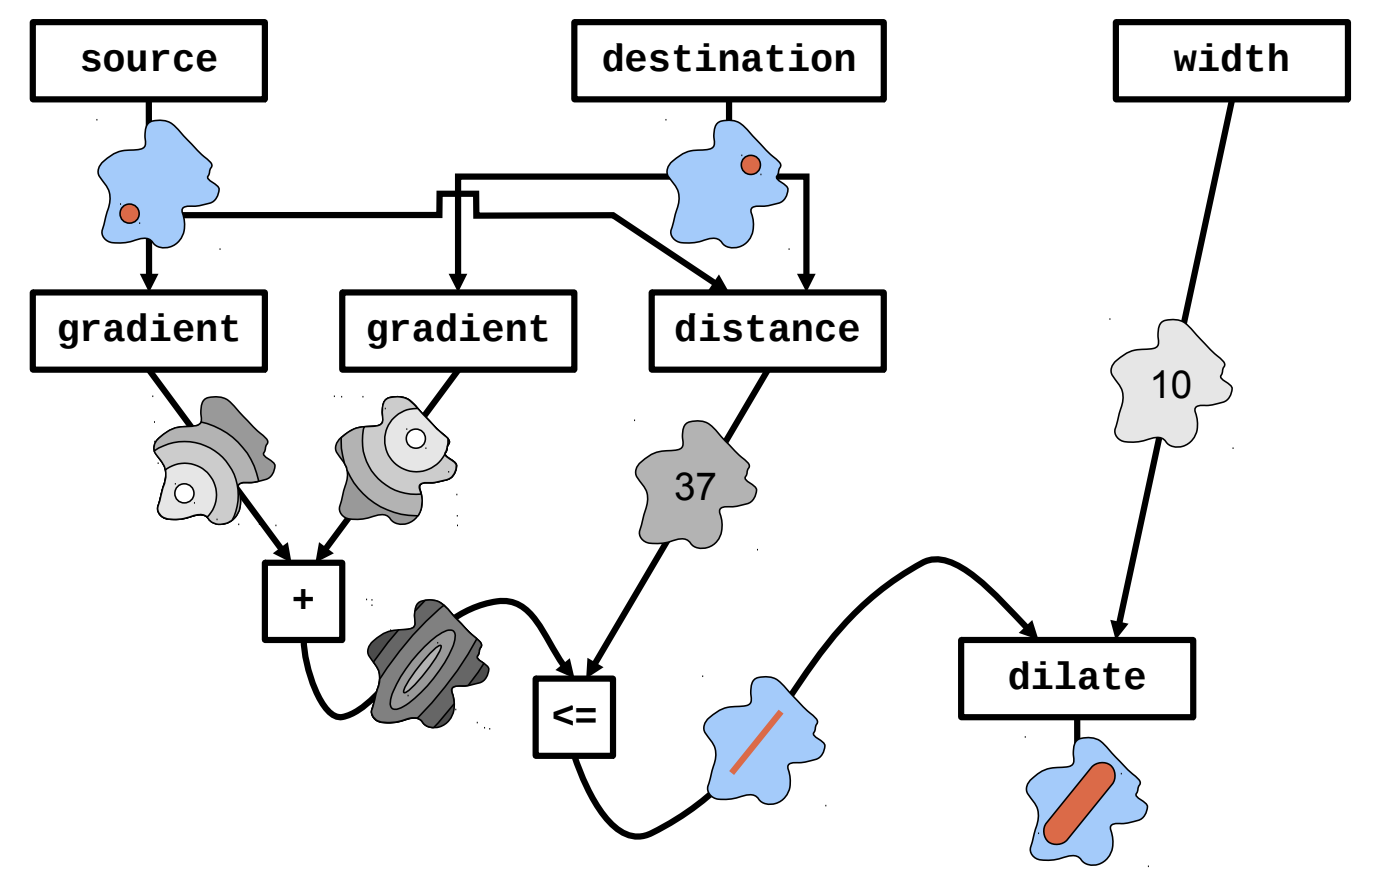
\includegraphics[width=0.7\textwidth]{figures/channel.png}
        \caption{Channel example}
        \label{fig:channel}
      \end{figure}

      \lstinputlisting[float,language=Scala,label={lst:channel-code}]{listings/Channel.scala}

%
\section{Reinforcement Learning}
%
\section{Multi-Agent Reinforcement Learning}

%----------------------------------------------------------------------------------------
\chapter{Requirements} 
\label{chap:requirements}
%----------------------------------------------------------------------------------------


%----------------------------------------------------------------------------------------
\chapter{Design} 
\label{chap:design}
%----------------------------------------------------------------------------------------


%----------------------------------------------------------------------------------------
\chapter{Implementation} 
\label{chap:implementation}
%----------------------------------------------------------------------------------------


%----------------------------------------------------------------------------------------
\chapter{Validation} % possible chapter for Projects
\label{chap:validation}
%----------------------------------------------------------------------------------------


%----------------------------------------------------------------------------------------
\chapter{\conclusionsname}
\label{chap:conclusions}
%----------------------------------------------------------------------------------------


%----------------------------------------------------------------------------------------
% BIBLIOGRAPHY
%----------------------------------------------------------------------------------------

%\nocite{*} % uncomment this to show all the reference in the .bib file
\bibliographystyle{plain}
\bibliography{bibliography}


\end{document}